\onecolumn
\section{Ablation Study with Memory Constraints} \label{sec:memory}

\begin{table}[!h]
    \small
    \centering
    \begin{tabular}{ccccccc}
        \toprule
        \bf Backprop Len & \bf Recurrence & \bf Encoding & \bf Loss & \bf pplx best & \bf pplx init & \bf Attn Len \\
        \midrule
        128 & \cmark & Ours & Full & \textbf{26.77} & \textbf{27.02} & \textbf{500} \\
        128 & \cmark & Ours & Partial & 28.33 & 28.69 & 460 \\
        \midrule
        176 & \xmark & Ours & Full & 27.98 & 28.43 & 400 \\
        172 & \xmark & Ours & Partial & 28.83 & 28.83 & 120 \\
        \bottomrule
    \end{tabular}
    \caption{\small
        Ablation study on WikiText-103 with the same GPU memory constraints.
    }
    \label{table:memory}
\end{table}

Table \ref{table:memory} compares Transformer-XL with baseline under the same memory budget. Transformer-XL still outperforms the baseline even with a shorter backprop length.

\section{Efficient Computation of the Attention with Relative Positional Embedding}
\label{sec:A-efficient-attention}
As we discussed in section \ref{sec:rel-pos-embed}, the naive way of computing the $\rmW_{k,R} \rmR_{i-j}$ for all pairs $(i, j)$ is subject to a quadratic cost.
Here, we present a simple method with only a linear cost.
Firstly, notice that the relative distance $i - j$ can only be integer from 0 to $M+L-1$, where $M$ and $L$ are the memory length and segment length respectively.
Hence, the rows of the matrix
\[\small
	\rmQ
	\coloneqq \begin{bmatrix} \rmR_{M+L-1}^\top \\ \rmR_{M+L-2}^\top \\ \vdots \\ \rmR_{1}^\top \\ \rmR_{0}^\top \end{bmatrix} {\rmW_{k,R}}^\top
	= \begin{bmatrix}
		\left[ \rmW_{k,R} \rmR_{M+L-1} \right]^\top \\
		\left[ \rmW_{k,R} \rmR_{M+L-2} \right]^\top \\ \vdots \\
		\left[ \rmW_{k,R} \rmR_{1} \right]^\top \\
		\left[ \rmW_{k,R} \rmR_{0} \right]^\top \end{bmatrix}
	\in \R^{(M+L) \times d}
\]
consist of all possible vector outputs of $\rmW_{k,R} \rmR_{i-j}$ for any $(i, j)$.
Note that we have defined $\rmQ$ in a reversed order, i.e., $\rmQ_k = \rmW_{k,R} \rmR_{M+L-1-k}$, to make further discussion easier.

Next, we collect the term $(b)$ for all possible $i, j$ into the following $L \times (M+L)$ matrix,
\begin{align*}
\rmB &=
	\begin{bmatrix}
	q_0^\top \rmW_{k,R} \rmR_{M}   & \cdots & q_0^\top \rmW_{k,R} \rmR_{0} & 0 & \cdots & 0 \\
	q_1^\top \rmW_{k,R} \rmR_{M+1} & \cdots & q_1^\top \rmW_{k,R} \rmR_{1} & q_1^\top \rmW_{k,R} \rmR_{0} & \cdots & 0 \\
	\vdots & \vdots & \vdots & \vdots & \ddots & \vdots \\
	q_{L-1}^\top \rmW_{k,R} \rmR_{M+L-1} & \cdots & q_{L-1}^\top \rmW_{k,R} \rmR_{M+L-1} & q_{L-1}^\top \rmW_{k,R} \rmR_{L-1} & \cdots & q_{L-1}^\top \rmW_{k,R} \rmR_{0} \\
	\end{bmatrix} \\
	&=
	\begin{bmatrix}
	q_0^\top \rmQ_{L-1}   & \cdots & q_0^\top \rmQ_{M+L-1} & 0                       & \cdots & 0 \\
	q_1^\top \rmQ_{L-2}   & \cdots & q_1^\top \rmQ_{M+L-2} & q_1^\top \rmQ_{M+L-1}   & \cdots & 0 \\
	\vdots                & \vdots & \ddots                & \vdots                  & \ddots & \vdots \\
	q_{L-1}^\top \rmQ_{0} & \cdots & q_{L-1}^\top \rmQ_{M} & q_{L-1}^\top \rmQ_{M+1} & \cdots & q_{L-1}^\top \rmQ_{M+L-1} \\
	\end{bmatrix}
\end{align*}
Then, we further define
\[
	\widetilde{\rmB} = \rvq \rmQ^\top =
	\begin{bmatrix}
	q_{0}^\top \rmQ_{0}   & \cdots & q_{0}^\top \rmQ_{M}   & q_{0}^\top \rmQ_{M+1}    & \cdots & q_{0}^\top \rmQ_{M+L-1}   \\
	q_{1}^\top \rmQ_{0}   & \cdots & q_{1}^\top \rmQ_{M}   & q_{1}^\top \rmQ_{M+1}    & \cdots & q_{1}^\top \rmQ_{M+L-1}   \\
	\vdots                & \vdots & \ddots                & \vdots                   & \ddots & \vdots                    \\
	q_{L-1}^\top \rmQ_{0} & \cdots & q_{L-1}^\top \rmQ_{M} & q_{L-1}^\top \rmQ_{M+1}  & \cdots & q_{L-1}^\top \rmQ_{M+L-1} \\
	\end{bmatrix}.
\]
Now, it is easy to see an immediate relationship between $\rmB$ and $\widetilde{\rmB}$, where the $i$-th row of $\rmB$ is simply a left-shifted version of $i$-th row of $\widetilde{\rmB}$.
Hence, the computation of $\rmB$ only requires a matrix multiplication $\rvq \rmQ^\top$ to compute $\widetilde{\rmB}$ and then a set of left-shifts.

Similarly, we can collect all term $(d)$ for all possible $i, j$ into another $L \times (M+L)$ matrix $\rmD$,
\begin{align*}
	\rmD &=
	\begin{bmatrix}
	v^\top \rmQ_{L-1} & \cdots & v^\top \rmQ_{M+L-1} & 0 & \cdots & 0 \\
	v^\top \rmQ_{L-2} & \cdots & v^\top \rmQ_{M+L-2} & v^\top \rmQ_{M+L-1} & \cdots & 0 \\
	\vdots            & \vdots & \ddots              & \vdots              & \ddots & \vdots     \\
	v^\top \rmQ_{0}   & \cdots & v^\top \rmQ_{M}     & v^\top \rmQ_{M+1}   & \cdots & v^\top \rmQ_{M+L-1} \\
	\end{bmatrix}.
\end{align*}
Then, we can follow the same procedure to define
\[
\widetilde{\rvd} = \left[\rmQ v \right]^\top
	=
	\begin{bmatrix}
	v^\top \rmQ_{0}   & \cdots & v^\top \rmQ_{M}     & v^\top \rmQ_{M+1}   & \cdots & v^\top \rmQ_{M+L-1}
	\end{bmatrix}.
\]
Again, each row of $\rmD$ is simply a left-shift version of $\widetilde{\rvd}$.
Hence, the main computation cost comes from the matrix-vector multiplication $\widetilde{\rvd} = \left[\rmQ v \right]^\top$, which is not expensive any more.

\section{Details About RECL} \label{sec:recl}
\begin{figure}[!h]
	\begin{subfigure}[b]{0.5\textwidth}
		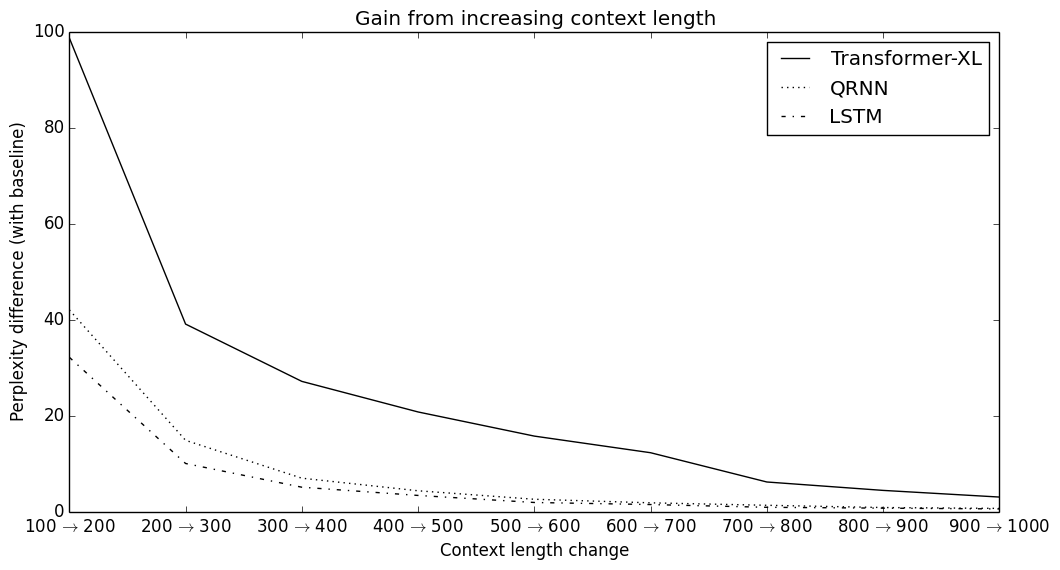
\includegraphics[width=\textwidth]{FIG/compare0.png}
		\caption{Transformer-XL vs RNNs}
		\label{fig:vsrnn}
	\end{subfigure}
	\begin{subfigure}[b]{0.5\textwidth}
		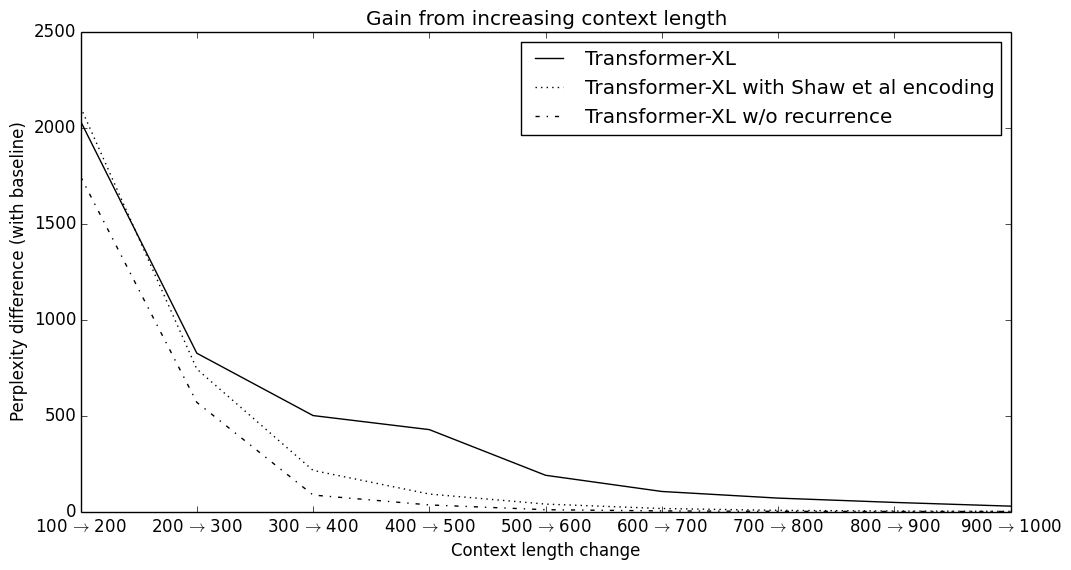
\includegraphics[width=\textwidth]{FIG/compare1.png}
		\caption{Transformer-XL vs Baseline}
		\label{fig:vsbase}
	\end{subfigure}
	\caption{Visualizing unnormalized relative perplexity gains with $r = 0.1$.}
	\label{fig:gain}
\end{figure}

\begin{figure}[!h]
	\begin{subfigure}[b]{0.5\textwidth}
		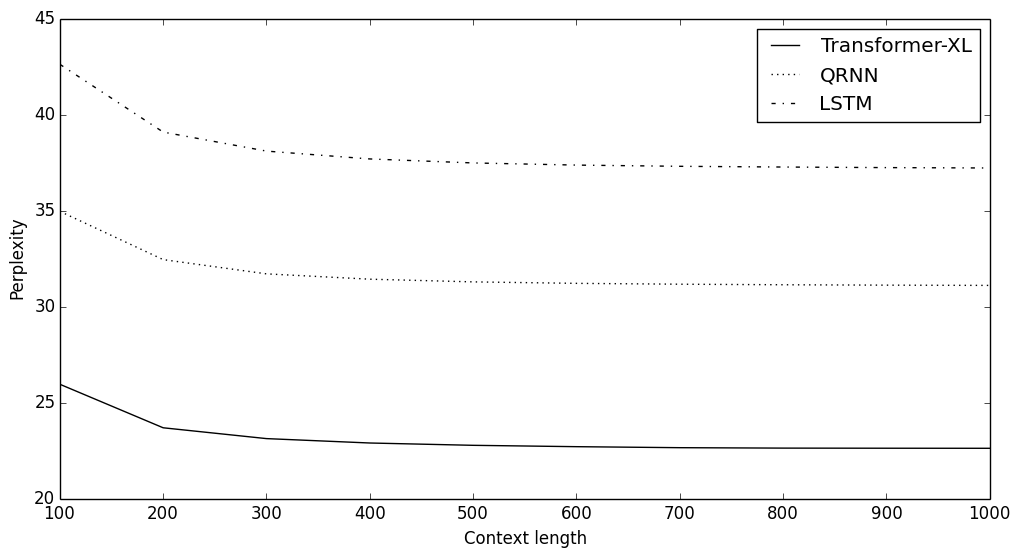
\includegraphics[width=\textwidth]{FIG/compare2.png}
		\caption{Transformer-XL vs RNNs}
		\label{fig:vsrnn}
	\end{subfigure}
	\begin{subfigure}[b]{0.5\textwidth}
		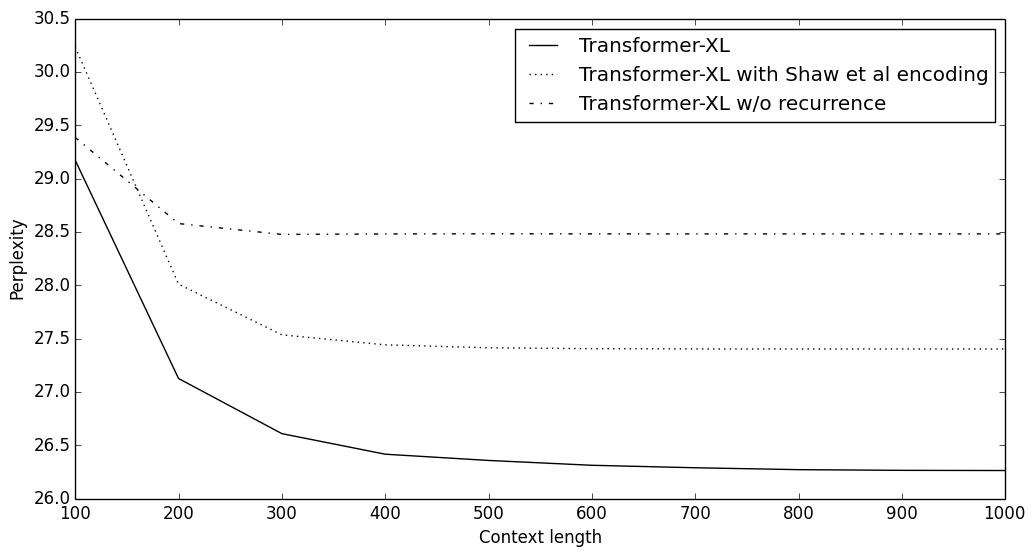
\includegraphics[width=\textwidth]{FIG/compare3.png}
		\caption{Transformer-XL vs Baseline}
		\label{fig:vsbase}
	\end{subfigure}
	\caption{Perplexity vs context length.}
	\label{fig:context}
\end{figure}

In this section, we describe the details of the metric RECL. Let $\mathcal{M} = \{m_1, m_2, \cdots, m_N\}$ be a model group consisting of $N$ models. Let $l_i(c, t)$ denote the loss of model $m_i$ on the $t$-th token in the corpus with a context length $c$. Concretely, the loss can be written as
\[
l_i(c, t) = - \log P_{m_i}(x_t | x_{t - 1}, \cdots, x_{t - c})
\]
where $P_{m_i}$ is the probability distribution given by model $m_i$, and $x_t$ is the $t$-th token in the corpus. Given a short context length $c$ and a long context length $c'$ such that $c' \geq c$, we can further define a baseline for each position $t$,
\[b(c, t) = \min_{i = 1}^N l_i(c, t)\]

The \textit{relative loss} of $m_i$ w.r.t. the model group $\mathcal{M}$ is written as
\[
f_i(c, c') = \frac{1}{|\mathcal{T}|} \sum_{t \in \mathcal{T}} \min \left( b(c, t), l_i(c', t) \right)
\]
The above equation uses the minimum loss of all models on the short length $c$ as a baseline, and only losses smaller than the baseline will be effectively counted towards the relative loss. This enables fair comparison between multiple models because all models with a long context length $c'$ need to improve over the same baseline. Sometimes we only care about those positions where the baseline performs poorly (which means short-term dependency with context length $c$ is not sufficient), so given a ratio parameter $r$, we define the set $\mathcal{T}$ is the above equation as
\[\mathcal{T} = \text{top-}r \text{~positions~} t \text{~with largest~}b(c, t)\]

The \textit{relative gain} is subsequently defined as the relative perplexity reduction:
\[
g_i(c, c') = \frac{\exp f_i(c, c) - \exp f_i(c, c')}{\exp f_i(c, c)}
\]

Given a step size $\Delta$, we then use an algorithm to find the RECL by thresholding the relative gain:
\begin{enumerate}
	\item Set initial short context length $c$, and long context length $c' = c + \Delta$
	\item Compute $g_i(c, c')$. If $g_i(c, c') < 0.01$, return $\text{RECL} = c$. If $g_i(c, c') \geq 0.01$, set $c = c', c' = c + \Delta$ and go to step 1.
\end{enumerate}

In Figure \ref{fig:gain}, we visualize the unnormalized relative perplexity gains $(\exp f_i(c, c) - \exp f_i(c, c'))$ with various pairs of $(c, c')$ when $r = 0.1$. It is clear that Transformer-XL has a longer RECL compared to RNNs and other baselines because the relative gains are substantially larger.

For reference, we plot the perplexities with varying context lengths in Figure \ref{fig:context}. The y-axis denotes the ``normal'' perplexity (not calibrated by baselines).

\section{Attention Visualization}
In this section, we provide some visualization of the attention learned by the SoTA model on the WikiText-103 validation set.
Recall that, this model has 16 10-head transformer layers and relies on a memory of length 640.

\begin{figure}[!h]
	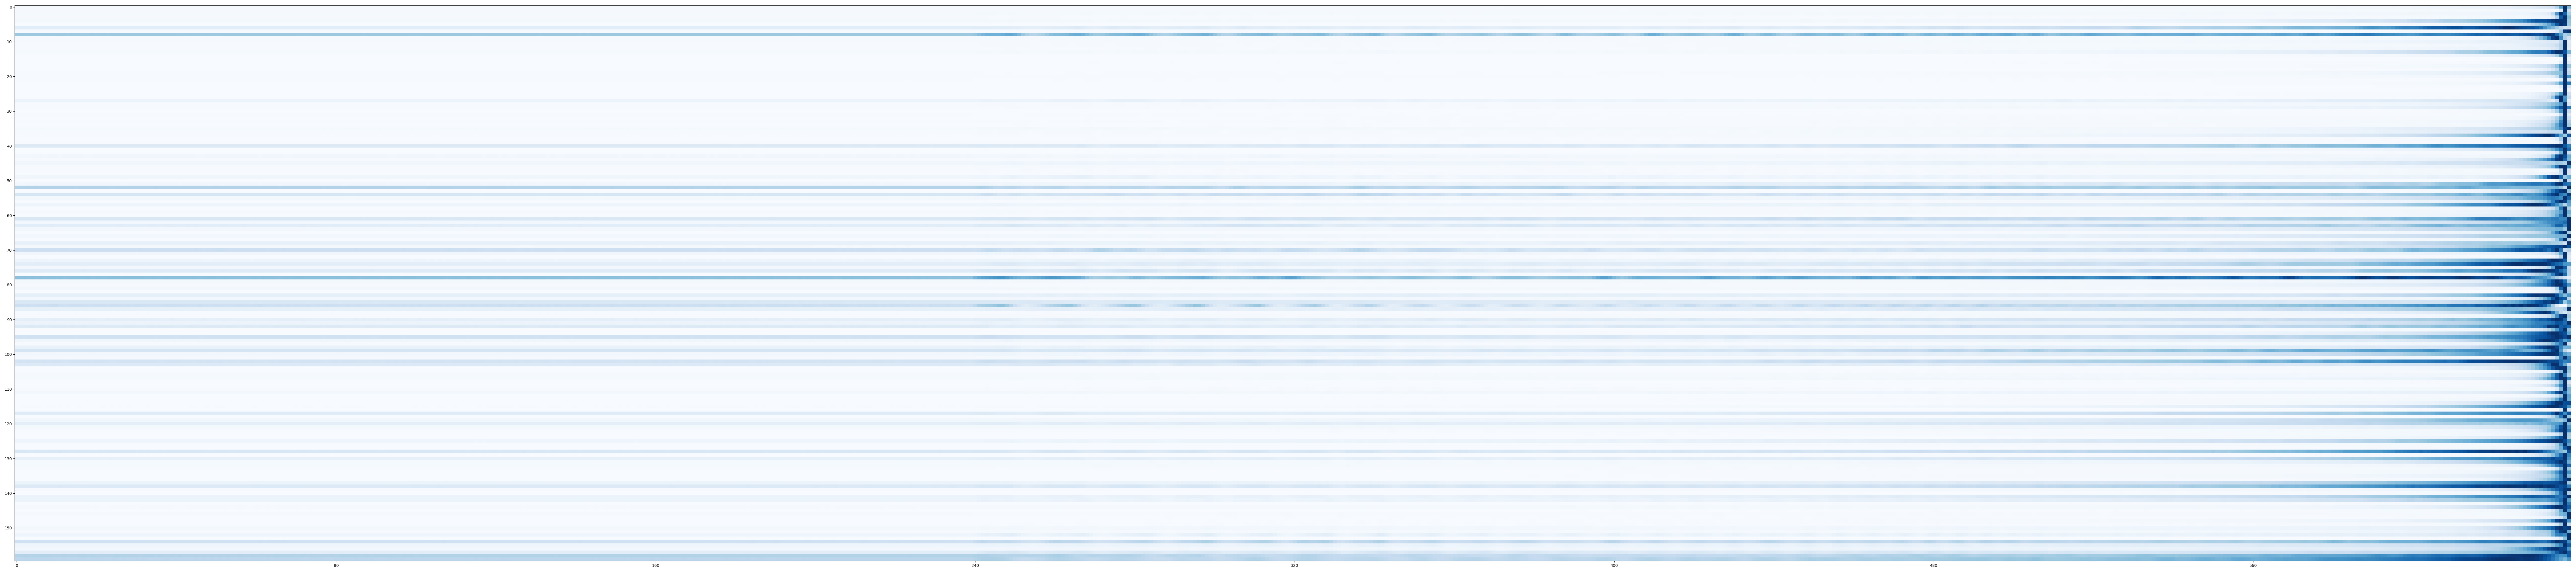
\includegraphics[width=\linewidth]{FIG/rel-prob-avg.png}
	\caption{Average attention over the previous 640 tokens, where each row corresponds to a attention head and each column corresponds to a relative location. There are totally 160 attention heads, and every 10 heads come from a single layer. Darker colors indicate higher values.}
	\label{fig:visattn-global}
\end{figure}
The first visualization aims at revealing the overall trend of where the model is attending.
Specifically, for each attention head of each layer, we average the attention distributions of all tokens in the validation set.
This is shown in Fig. \ref{fig:visattn-global}. As we can see, the overall trend is to focus more on the nearby tokens than the faraway ones.
However, it is also very clear that some attention heads have a wider attention distribution over the entire memory span, notably the head 8 from layer 1, head 78 from layer 8, and the head 158 from layer 16.

\begin{figure}[!h]
	\begin{subfigure}[b]{\linewidth}
		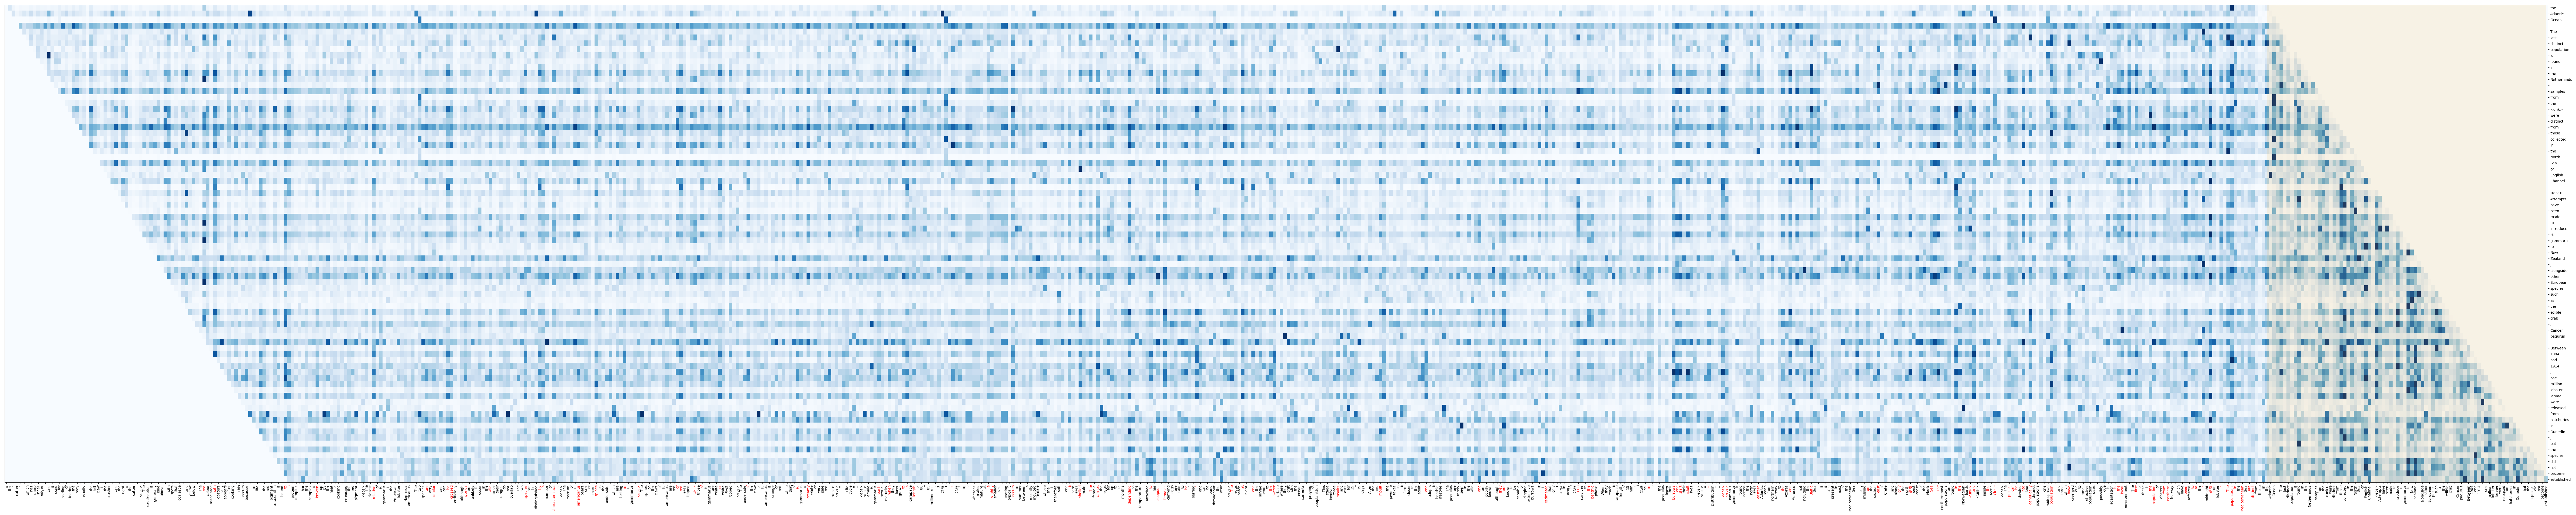
\includegraphics[width=\textwidth]{FIG/abs-prob-H8-seg4.png}
		\caption{Head 8 from layer 1.}
		\label{fig:visattn-8}
	\end{subfigure}
	\begin{subfigure}[b]{\linewidth}
		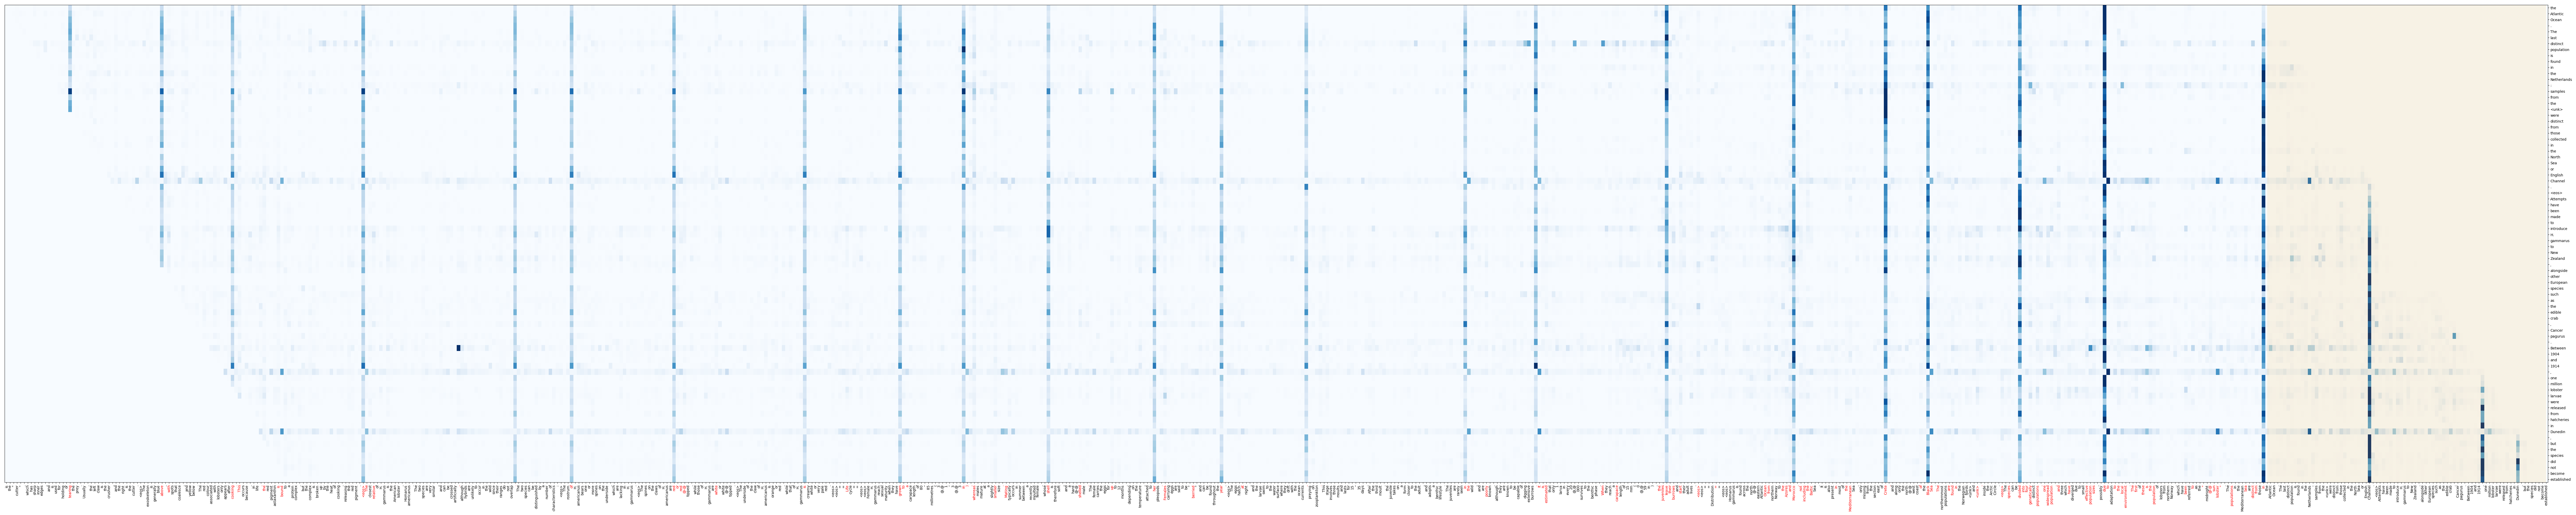
\includegraphics[width=\textwidth]{FIG/abs-prob-H78-seg4.png}
		\caption{Head 78 from layer 8.}
		\label{fig:visattn-78}
	\end{subfigure}
	\begin{subfigure}[b]{\linewidth}
		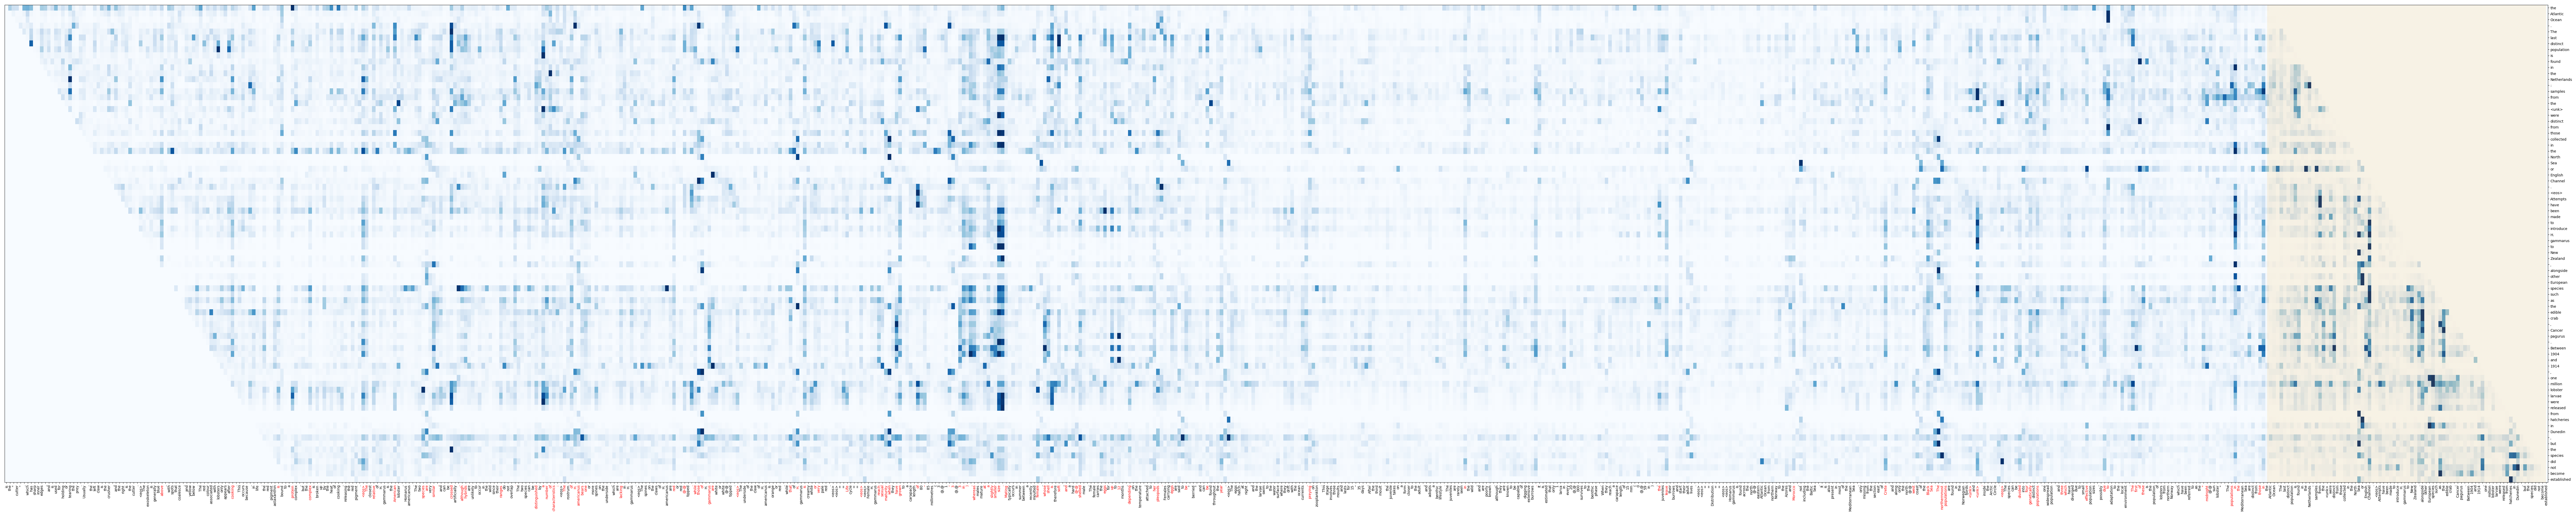
\includegraphics[width=\textwidth]{FIG/abs-prob-H158-seg4.png}
		\caption{Head 158 from layer 16.}
		\label{fig:visattn-158}
	\end{subfigure}
	\caption{Visualization of the three heads with a wide attention range. Each row corresponds to a target location/token and each column corresponds to a context location/token. Tokens in the memory that have top 20\% attention values are highlighted in red.}
	\label{fig:visattn-pick}
\end{figure}
Since we are focused on learning long-range dependency, we are especially interested in these heads with a wider attention span.
Thus, in the second set of visualization, we pick the three notable heads mentioned above, and visualize their attention behavior for a randomly chosen position, as shown in Fig. \ref{fig:visattn-pick}.
Here, we see three different patterns of wider attention:
\begin{itemize}[leftmargin=*]
	\item For the head 8 in the 1st layer, we see an almost uniform attention over the entire memory span. This is quite intuitive, as lower-level layers needs to screen the entire memory span to decide where to focus for higher-level layers
	\item For the head 78 in the 8th layer (a middle-level layer), we see a very sparse attention pattern scattered in all ranges of the memory. Again, this well fits our intuition that as information accumulates, the network may focus on some particular position with special interests.
	\item For the head 158 in the 16th layer (i.e. the last layer), each target location (corresponding to each row) has its own distinct sparse focus, differing from head 78 where target locations largely share the same attentive location in memory. Meanwhile, the pattern is also different from the case of head 8, where a few locations are clearly attended more than others.
\end{itemize}

\begin{figure}[!h]
	\begin{subfigure}[b]{\linewidth}
		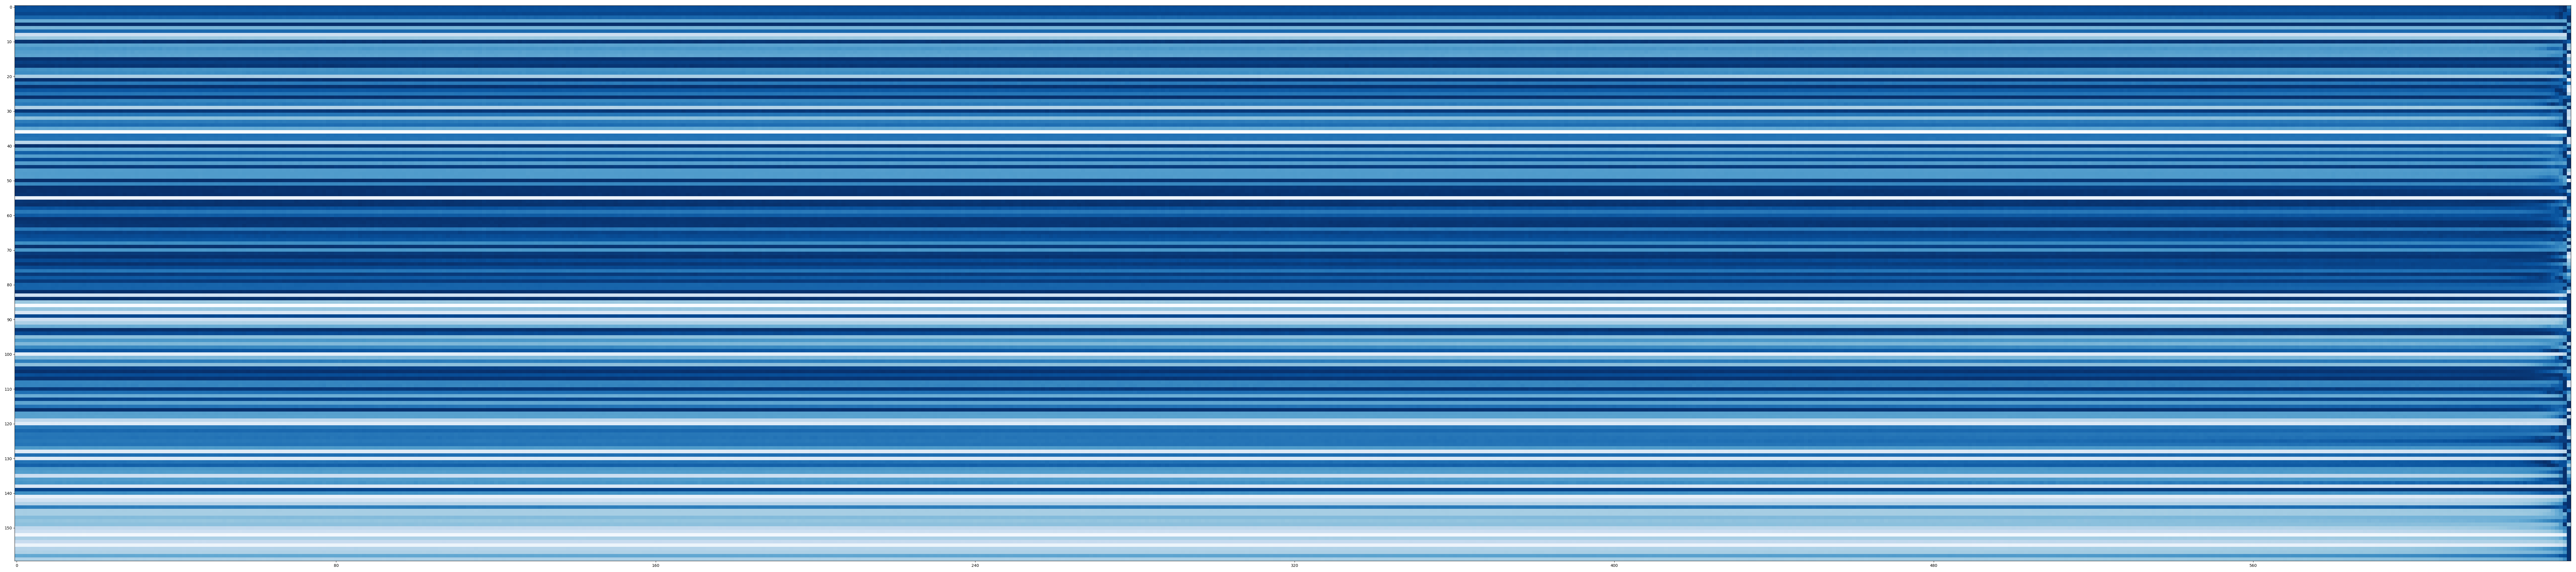
\includegraphics[width=\textwidth]{FIG/rel-A-avg.png}
		\caption{Term $(a)$.}
		\label{fig:visattn-A}
	\end{subfigure}
	\begin{subfigure}[b]{\linewidth}
		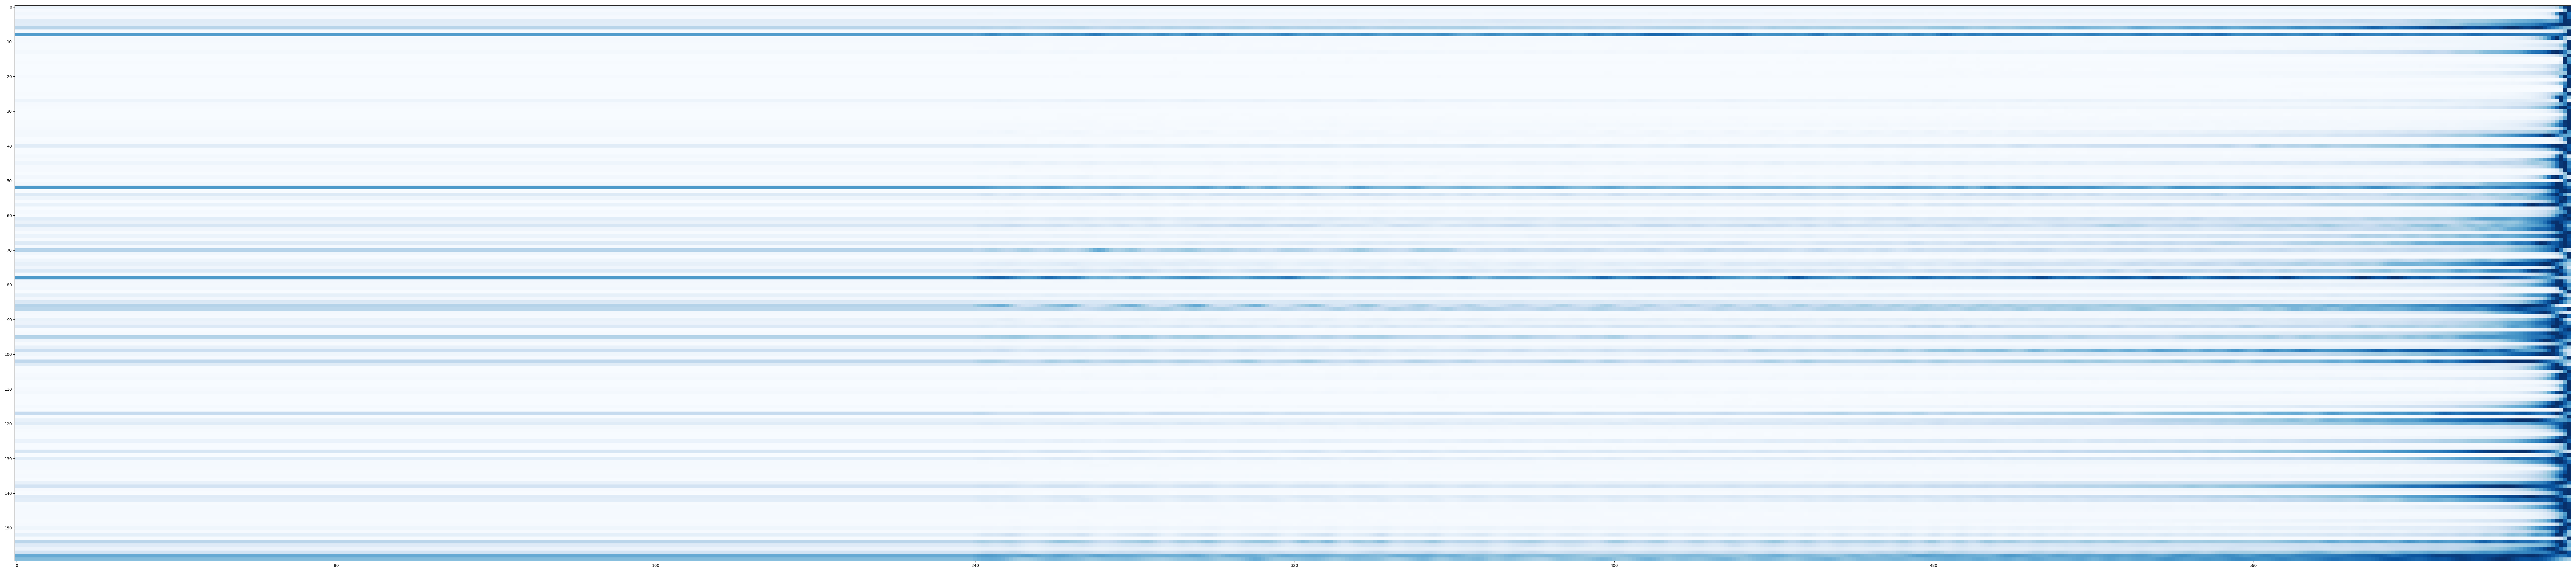
\includegraphics[width=\textwidth]{FIG/rel-B-avg.png}
		\caption{Term $(b)$.}
		\label{fig:visattn-B}
	\end{subfigure}
	\begin{subfigure}[b]{\linewidth}
		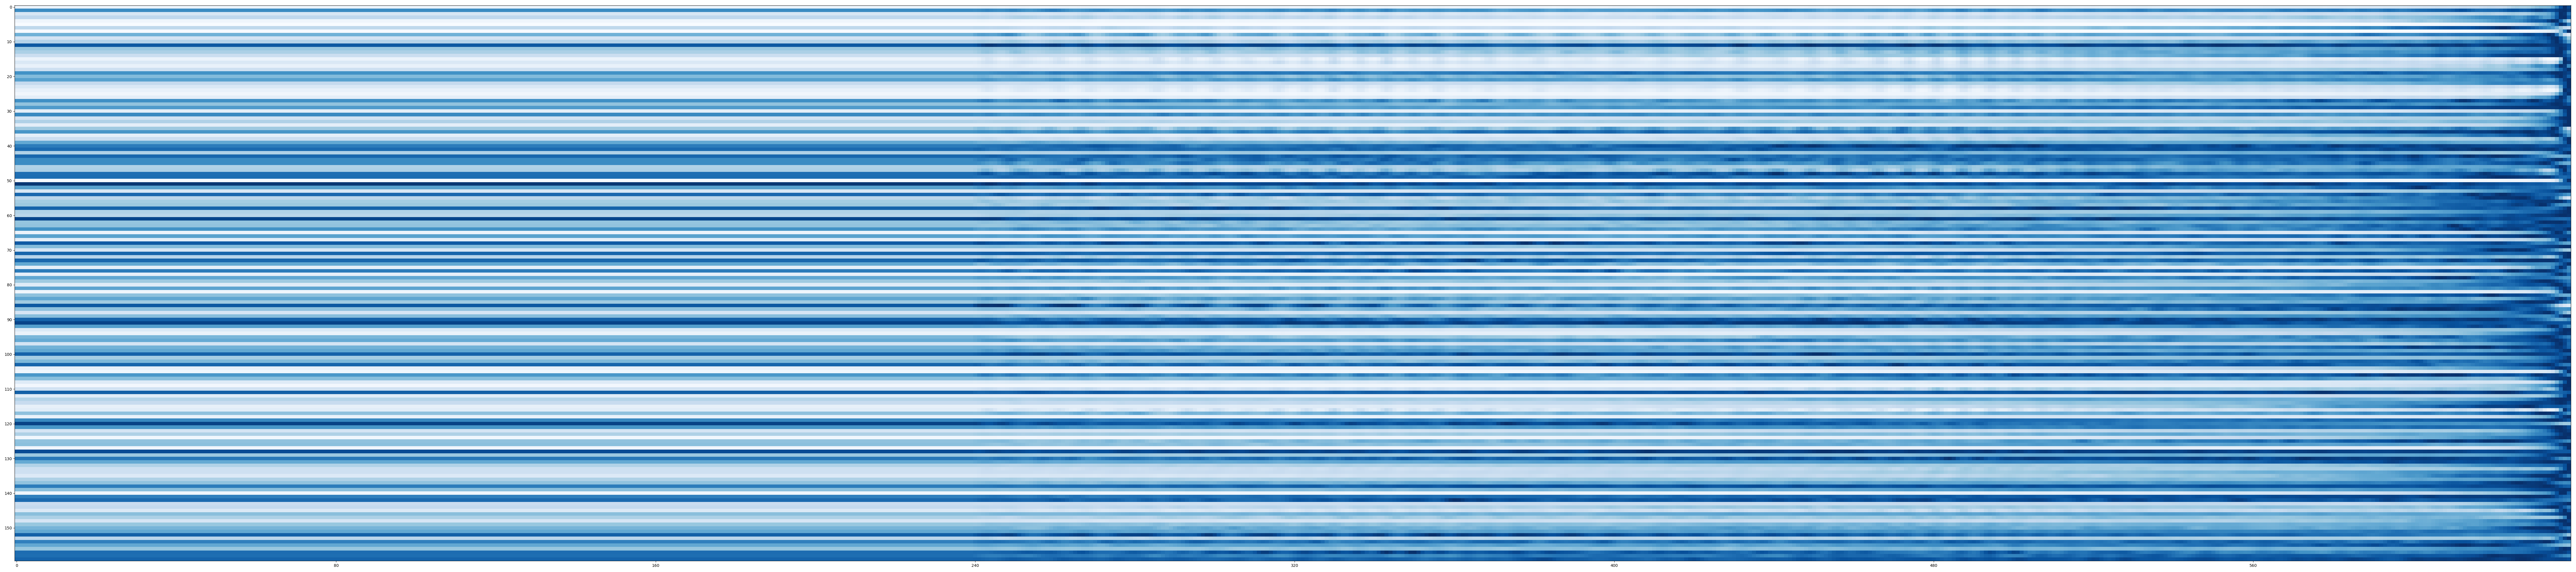
\includegraphics[width=\textwidth]{FIG/rel-D-avg.png}
		\caption{Term $(d)$.}
		\label{fig:visattn-D}
	\end{subfigure}
	\caption{Visualization of the three terms in computing the attention score. Each row corresponds to a attention head and each column corresponds to a relative location.}
	\label{fig:visattn-decomp}
\end{figure}
Finally, as we have discussed in section \ref{sec:rel-pos-embed}, the attention score can be decomposed into four intuitive terms.
Here, we want to further investigate how these four terms contribute to the overall attention trend in Fig. \ref{fig:visattn-global}.
Since the term $(c)$ represents the global content bias, i.e., the prior importance of each word regardless of the context, we will leave it out and focus on the terms $(a)$, $(b)$ and $(d)$.
So, for each term, we take the Softmax w.r.t. the memory span and average the resulted distribution of all tokens in the validation set.
The results are visualized in Fig. \ref{fig:visattn-decomp}:
\begin{itemize}[leftmargin=*]
	\item Since term $(a)$ is fully content-based addressing, when averaging over all target words, the result is essentially uniform over the entire context, except for a few very close words, which are likely to be semantically similar to the target word.
	\item The overall trend of term $(b)$ highly resembles that of the entire attention distribution in Fig. \ref{fig:visattn-global}. It suggests that the global trend of focusing on the nearby context is largely contributed by this content-dependent positional bias.
	\item The overall trend of term $(d)$ is also focusing more on nearby words. However, compared to the trend of term $(b)$, it is clearly flatter and biases towards a longer context.
\end{itemize}

\section{Generated Text} \label{sec:gen}
In this section, we present some generated text from our best model trained the Wikitext-103 dataset.
We seed the our Transformer-XL with a context of at most 512 consecutive tokens randomly sampled from the test set of Wikitext-103. Then, we run Transformer-XL to generate a \textit{pre-defined} number of tokens (500 or 1,000 in our case). For each generation step, we first find the top-40 probabilities of the next-step distribution and sample from top-40 tokens based on the re-normalized distribution.
To help reading, we detokenize the context, the generated text and the reference text. Three generated examples are shown in Tables \ref{tab:gen-1}, \ref{tab:gen-2}, and \ref{tab:gen-3}. Note that we do not perform any cherry picking and present the first three examples we generate in the paper.
In the text, ``= text ='', ``= = text = ='' and ``= = = text = = ='' denote the Wikipedia page tile, section title and subsection title, respectively, due to the original data preprocessing procedure of Wikitext-103~\cite{merity2016pointer}. 

%As we can see, though only trained on 100M tokens, Transformer-XL is able to generate long text which structurally maintains the sectional arrangement of Wikipedia and semantically stays on the same topic as the seed context.
%It is clear that important information is carried over the course of generation by Transformer-XL, which demonstrates the ability of long-range dependency modeling.
%For detailed explanation of the interesting observations in each example, please refer to the corresponding caption.
%
%Despite the overall excellence of the generation quality, there are some typical detectable flaws in the generated text:
%\begin{itemize}
%\item Firstly, the model can only perceive the seed context and hallucinate the generation based on the limited knowledge (100M tokens only) it is trained on. As a result, the generated text sometimes looks clearly relevant but not close enough or to the point compared to what human writer would do. 
%That said, we believe this issue is mostly a problem of the limited training data size. 
%
%\item Secondly, the model might generate text with repetitive or contradictory information, e.g., the same or slightly different message is expressed multiple times, though with potentially different forms. This issue can also be possibly resolved by training on more data.
%\end{itemize}

As we can see, though only trained on 100M tokens, Transformer-XL is a strong model at generating long text articles, particularly in the following aspects:
\begin{itemize}[topsep=0em,itemsep=0em,parsep=0.2em]
	\item Transformer-XL is able to structurally maintain the sectional arrangement of Wikipedia.
	\item Transformer-XL manages to semantically stay on the same topic throughout the course of generation.
	\item Long-range references are common in the generated text.
	\item Transformer-XL often generates novel content that is not present in the training data.
\end{itemize}
For more detailed explanation of the interesting observations in each example, please refer to the corresponding caption.

Despite the overall excellence of the generation quality, the model can only perceive the seed context and hallucinate what to generate based on the limited knowledge (100M tokens only) it is trained on. As a result, the generated text sometimes looks clearly relevant but not close enough or to the point compared to what human writer would do. 
That said, we believe this issue is mostly a problem of limited training data size and could be alleviated by using a larger training set.

\begin{table}[!h]
\centering
\scriptsize
%\begin{adjustwidth}{-0.8cm}{}
\begin{tabular}{p{7.8cm}|p{7.8cm}}
	\toprule
	\multicolumn{2}{p{16cm}}{\textbf{Context:}} \\
	\multicolumn{2}{p{16cm}}{Kershaw started the 2010 season by posting a 3.07 ERA in April, but did so by walking 22 batters in 29 innings. On May 4, he had his worst start of his career against the Milwaukee Brewers at Dodger Stadium, throwing just 57 pitches in 11 / 3 innings, while retiring only four of the 13 batters he faced — including the pitcher. He was booed loudly upon being pulled from the game. Kershaw said after the game, " I didn't give our team any kind of chance. It's just not a good feeling to let your teammates down, let everybody down. It stings, it hurts. I 've got to figure things out. " 
Kershaw rebounded his next start by pitching an 8 inning two-hitter and out-dueling the then undefeated Ubaldo Jim\'{e}nez. He credited his control of the slider being the major turning point for him. Later in the season, he was suspended for five games after hitting Aaron Rowand of the Giants with a pitch in a game on July 20. The incident occurred after both teams were given a warning following Giants ace Tim Lincecum hitting Matt Kemp earlier in the game. He threw his first career complete game shutout on September 14, 2010 also against San Francisco and finished the season with a record of 13 – 10 and a 2.91 ERA in 32 starts, pitching 2041 / 3 innings and recording 212 strikeouts. 

= = = = 2011 season: 1st Cy Young Award = = = = 

After finishing the 2010 season strong, the Dodgers named Kershaw as the Opening Day Starter for the 2011 season. On May 29, he pitched the second complete-game shutout of his career, striking out 10 while winning a two-hitter against the Florida Marlins, 8 – 0; he also had two singles and an RBI, scoring twice in the game. He produced his third career shutout on June 20, a two-hit, 11-strikeout effort against the Detroit Tigers. Kershaw became the first Dodgers starter to strike out the side in the 9th inning since Sandy Koufax's perfect game. In his next start, on June 26, Kershaw pitched another complete game (against the Los Angeles Angels of Anaheim ). He became the first Dodger starter to have back-to-back complete game victories since Jeff Weaver in the 2005 season and the first Dodger to have double-digit strikeouts in consecutive starts since Chan-Ho Park in the 2000 season. He was awarded the National League Player of the Week award for the week of June 20 – 26 as a result of those two starts. Midway through June, Kershaw had amassed 32 career victories } \\
	\midrule
	\textbf{XL Generation:} & \textbf{Reference:} \\	
	, tying him with Luis Castillo for the third best start total in the league and trailing only Johnny Bench and Eddie Mathews (37). The Dodgers signed Kershaw to a one-year deal on July 14, 2011, with a player option for 2012, in a deal worth just under \$ 300,000. 
The Dodgers entered the 2011 season as the major league leaders, and Kershaw had the best record in the National League in saves (39), games started (78) and walks (120); he also had the lowest win / loss ratio in the league (1.87), and he had the worst on-base percentage (.349). He had the best ERA (2.00 ), most wins (16 ), or most shutouts (29) in his career (25), while leading the league in losses per nine innings pitched (4.01). Following the 2011 season, the Dodgers traded Kershaw to the Kansas City Royals on July 29 for pitcher Javier Torres. 

= = = Kansas City Royals = = = 


= = = = 2012 season = = = = 

During spring training, Kershaw played very well. He was selected to spring training as a relief pitcher for the Royals for the 2012 season. After an injury to closer Javier Vázquez, he was activated on April 29 to replace Matt Holliday in the Royals ' starting rotation. In his only start with the Royals, on August 6, 2012, Kershaw struck out five batters in seven innings pitched to help the Royals to their first victory in franchise history. On September 27, 2012, it appeared Kershaw was going to pitch a complete game shutout against the Detroit Tigers, but did not manage to do so since the Tigers won 3 – 1. At the conclusion of the season, Kershaw was named Major League Baseball's Most Valuable Player, was chosen to the All-Star Game at Busch Stadium and was named to the All-Star Game as the starting pitcher at shortstop. The Royals announced on February 4, 2013 that Kershaw would spend 2013 as starting pitcher, though he was expected to miss the season as a result of a shoulder injury. 

= = = = 2013 season = = = = 

On May 17, 2013, Kershaw sustained \underline{another back injury} and did not start in August and October 2013. He appeared in 22 starts, all starts, finishing with a strikeout-to-walk ratio of 1.50 and a 2.91 ERA. He also had the third most strikeouts in the league: 10. On May 20, 2013, he & , a 3.15 ERA and 593 career strikeouts in 568.2 innings. According to the Elias Sports Bureau, Kershaw was the first 23-year-old pitcher to have that many victories, an ERA that low and an average of more than one strikeout per inning since ERA became an official statistic in 1910. 
Kershaw was selected to the National League team for the 2011 Major League Baseball All-Star Game, his first All-Star selection. In the month of July, Kershaw was 4 – 1 with a 2.02 ERA and NL-leading 45 strikeouts, earning him the National League Pitcher of the Month Award. On August 23, he struck out Matt Holliday of the St. Louis Cardinals for his 200th strikeout of the season and became the 10th Dodger pitcher to record back-to-back 200 strikeout seasons and the first since Chan-Ho Park did it in the 2001 season. 
Kershaw finished the 2011 season by leading the NL with 21 wins, 248 strikeouts and a 2.28 ERA, winning the NL pitching Triple Crown, the first Triple Crown winner since Jake Peavy of the 2007 San Diego Padres and the first Dodger since Sandy Koufax won it in the 1966 season. Justin Verlander of the Detroit Tigers won the American League Triple Crown the same season, marking the first major-league season since 1924 to feature Triple Crown-winning pitchers in both leagues. Kershaw's 21 wins were the most by a Dodger pitcher since Orel Hershiser won 23 during the 1988 season. His ERA was the lowest by a Dodger since Hershiser's 2.03 in the 1985 season, his strikeouts were the most by a Dodger since Koufax's 317 in 1966 and his 233 1 / 3 innings pitched were the most since Chan Ho Park pitched 234 in 2001. Since 1965 when Koufax did it, Peavy and Kershaw are only two pitchers in the National League have led the league in wins, strikeouts, ERA, and WHIP (walks plus hits per inning pitched). Kershaw also became just the second <unk> to have a 240-plus strikeouts in a season before the age of 24, joining Vida Blue. 
After the season, Kershaw was awarded the Warren Spahn Award as the best left-handed pitcher in 2011, the Players Choice Award for Most Outstanding National League pitcher, the Gold Glove Award as the top fielding pitcher in the NL and the Sporting News (TSN) National League Pitcher of the Year. He was additionally selected as the starting pitcher for the TSN NL All-Star Team. On November 17, he was honored with the National League Cy Young Award, making him the youngest Cy Young winner since Dwight Gooden 
 \\
	\bottomrule
\end{tabular}
\captionsetup{singlelinecheck=off}
\caption[]{\small 
	Example 1 -- 500 tokens generated by XL using a snippet from the Wikitext-103 test set as initial context. The sample is randomly generated without any cherry picking. 
	\vspace{0.4em}
	
	Original Wikipedia page: {\footnotesize \url{https://en.wikipedia.org/wiki/Clayton_Kershaw}}
	\vspace{0.4em}
	
	There are many interesting observations from this example:
	\begin{itemize}[leftmargin=*,itemsep=0em,topsep=0.4em,parsep=0.4em]
		\item Firstly, Kershaw never went to Royals in real life. Despite that, Transformer-XL stays on the fully imagined topic and keeps hallucinating the experience of Kershaw in Royals across the generated text.
		\item Secondly, notice that XL correctly tracks the chronological order from 2011 to 2012 and to the finally 2013 season in the section titles. 
		\item  In addition, notice that Transformer-XL accurately uses the the phrase ``\underline{another back injury}'' in the 2013 season paragraph, since it has talked about one earlier injure in the 2012 season. This shows again Transformer-XL's ability of capturing long-term dependency.
	\end{itemize}
}
\label{tab:gen-1}
%\end{adjustwidth}
\end{table}

\begin{table}[!h]
\centering
\scriptsize
\begin{tabular}{p{7.8cm}|p{7.8cm}}
	\toprule
	\multicolumn{2}{p{16cm}}{\textbf{Context:}} \\
	\multicolumn{2}{p{16cm}}{= = Distribution = = 

Species range across the Neotropics from Mexico in the north to Bolivia, Paraguay, and southern Brazil in the south. According to <unk> and coauthors, three species are found in Mexico, four in Central America, and 62 in South America. Three species are present in the Caribbean — two in Trinidad and Tobago, along the southern edge of the region, and one in Haiti. 

= = Habitat and ecology = = 

<unk> includes both large trees and small acaulescent palms which occupy a number of different ecological niches. Dense stands of some of the larger species are conspicuous elements on the landscape, while smaller species are found in both in the forest understorey and in savannas. 
Disturbance has been implicated in the formation of vegetation dominated by large <unk> species. In seasonally dry Amazonian forests the density of large adult A. <unk> palms was correlated with canopy openness; the species also dominates savannas formed by repeated forest fires in Trinidad and Tobago. <unk> speciosa forms pure stands in many parts of Brazil where natural forest vegetation has been cleared. Similarly, stands of A. <unk> in Bahia, Brazil (which are cultivated for <unk> fibre) are managed using fire — the seedlings survive cutting and burning, and are able to dominate burned forest patches. 
The fruit are dispersed by animals; fruit which are not dispersed frequently suffer seed predation by <unk> beetles. Certain species of <unk> have been mentioned as examples of " anachronistic " species which are adapted for dispersal by now-extinct Pleistocene megafauna. On <unk> Island, <unk>, in the Brazilian Amazon, <unk> <unk> fruit were consumed by tapirs, collared peccaries, deer and primates. Rodents, including agoutis, fed upon the fruit and, as the fruit availability declined, they fed on the seeds. Other dispersers of <unk> fruit include Crested <unk> which consume the fruit and disperse the seeds of A. <unk> in the Brazilian Pantanal. 

= = Uses = = 

<unk> species have a long history of human utilisation. <unk> <unk> <unk> seeds have been found in archaeological sites in Colombia dating back to 9000 BP. A variety of species remain important sources of edible oil, thatch, edible seeds and fibre. The leaves of <unk> <unk> and A. <unk> are used extensively for thatching. Several species are oil palms, with A. speciosa among the most important economically. Products extracted from A. speciosa were reported to support over 300,000 households in the Brazilian state of Maranhão in 2005, and in 1985 it was estimated to support over 450,000 households throughout the Brazil. <unk> fibres, extracted from the leaf bases of A. <unk>, are commercially important, and generated about US \$} \\
	\midrule
	\textbf{XL Generation:} & \textbf{Reference:} \\	
	700,000 in 2013 on the black market. In 2004 the plant was reported to be responsible for a net profit of around US \$ 3 million in Brazil. A 2012 study found A. speciosa to cause agricultural production at least 2 – 3 times greater than those achieved without prior knowledge of land management. 


\underline{= The Tale of Mrs. Tittlemouse =}

The Tale of Mrs. Tittlemouse is a children's book written and illustrated by H. M. Potter. It was first published in February 1910 by Frederick Warne \& Co. and included illustrations by Frederick Warne. Mrs. Tittlemouse was intended to be a children's book, rather than a musical, and the tale describes her attempts to find her own home. Mrs. Tittlemouse is an average kitten and the tale follows a mischievous rabbit named Mr. Tittlemouse who tries to kill her in an attempt to get a ride on a horse. Potter later wrote of the rabbit and her attempts to kill her, " If [ she ] were a fox, I should like to have been able to show her the way. " 
Potter's work was inspired by The Tale of Little Black Sambo and her two nieces, Petunia and Petunia. It was the first book in the Potter family to be published in a hardback format, and was also the first book in the Peter Rabbit series. The tale was released on 13 November 1910 and was accompanied by a greeting card by Potter's brother-in-law, Frederick Warne. 
The tale was well received by critics and children, and sold over 600,000 copies in its first few years. In the first year of its publication, Potter's The Tale of Mrs. Tittlemouse won children's book awards in England, America and Australia. It was selected as a " recommended reading " by children in the US and Canada. 

= = Plot summary = = 

The tale opens with the pet rabbit Mrs. Tittlemouse wandering through a forest in a small litter of four. He is shot and badly injured by a deer after she attempts to escape. Mrs. Tittlemouse decides that she wants to find her own home, because she is eager to go on her own. She goes alone to the farm where she makes a little money by selling a few seeds and building a small cabin in the woods. She is approached by a wealthy hunter named Mr. Tittlemouse, who tries to kill her but Mrs. Tittlemouse kills him by stuffing a rope into his nose and killing him. She is rescued by Mr. Tittlemouse's wife Ruth, but Mrs. Tittlemouse then leaves the woodland with the baby. When she is spotted by  & 20 million in annual income to Brazilian farmers in 1996. 


\underline{= The Heart of Ezra Greer =}

The Heart of Ezra Greer is a 1917 American silent drama film produced by the Thanhouser Company and directed by Emile <unk>. The film focuses on Ezra Greer, a successful middle-aged man who searches for his college age daughter, Mary. The wayward Mary was romanced and abandoned by Jack <unk>, later bearing his child. Once Ezra becomes broke he finds employment as the valet for Jack <unk>. After Jack's engagement to a cabaret girl, Mary becomes upset and leaves her child at Jack's home. Contrary to Jack's wishes, Ezra keeps the child and Jack ultimately reveals that the child is his own. Ezra convinces Jack to make things right and Ezra convinces the cabaret girl to leave Jack. After a carriage accident in which the baby is injured, Ezra and Jack rush to the hospital and find Mary as a nurse crying over the child. The film ends with the marriage of Jack and Mary. The film was released by Pathé on October 7, 1917. The film was the final release from Thanhouser and was deemed to be an average film by most reviewers. Criticism for the film hinged on far-fetched coincidences to drive the plot. The film is presumed lost. 

= = Plot = = 

The film follows Ezra Greer, a middle-aged man who has worked hard since his youth. He cares deeply for his motherless daughter, Mary, but was unable to attend the annual commencement at her co-educational college. He awaits for her to return from college, but Mary leaves with her romantic interest, Jack <unk>. On promise of marriage and wealth, Mary is romanced and gives birth to a fatherless child. Without word from his daughter, Ezra resigns from his job and attempts to seek her out and finds a poor motherless child, Marie. With Ezra's money exhausted he seeks employment and finds it as the valet of Jack. 
One day, Mary seeks an announcement of Jack's engagement to a cabaret girl known as " The Baby Vamp ". Bitter over the prospect of her child's future, she leaves the child at Jack's home during his absence with a note. Jack orders Ezra to take the baby to an orphanage, but Marie begs Ezra to keep him. After continually seeing the child, Jack is overcome with remorse and explains to Ezra and seeks his advice. Not knowing he was making the case for his own daughter, Ezra convinces Jack to seek out Mary and forget the Baby Vamp. The Baby  \\
	\bottomrule
\end{tabular}
\captionsetup{singlelinecheck=off}
\caption[]{\small 
	Example 2 -- 500 tokens generated by XL using a snippet from the Wikitext-103 test set as initial context. The sample is randomly generated without any cherry picking. 
	\vspace{0.4em}
	
	Original Wikipedia page: {\footnotesize \url{https://en.wikipedia.org/wiki/The_Tale_of_Mrs._Tittlemouse}}. \vspace{0.4em}
	
	This example exhibit some additional interesting properties of Transformer-XL: 
	\begin{itemize}[leftmargin=*,itemsep=0em,topsep=0.4em,parsep=0.4em]
		\item After finishing the last paragraph of the seed context, both the reference and generated text start a new topic (i.e., Wikipedia page), as marked by the single ``\underline{= title =}'' line. 
		This suggests the model has the ability of identifying the end of a topic / page, and randomly starting with a new topic.
		\item Even more interestingly, a newly-started page is on a book called ``The Tale of Mrs. Tittlemouse''. Transformer-XL manages to copy the same book title and some related information from the training set, but hallucinates \textit{novel} content of the book. 
		This demonstrates a degree of generalization instead of memorization. Please refer to the original book content at the Wikipedia page.
	\end{itemize}
}
\label{tab:gen-2}
\end{table}

\clearpage

%\begin{table}[!h]
%\centering
%\scriptsize
%\begin{adjustwidth}{-0.8cm}{}
\begin{center}
\scriptsize
\begin{longtable}{p{7.8cm}|p{7.8cm}}
	\toprule
	\multicolumn{2}{p{16cm}}{\textbf{Context:}} \\
	\multicolumn{2}{p{16cm}}{%<unk> undergo <unk> reactions with <unk> to afford a number of unique five membered <unk>, as depicted in the figure below. This reactivity is due to the strained three membered ring and weak N-O bond. 
= Battle of D\"{u}renstein = 

The Battle of D\"{u}renstein (also known as the Battle of <unk>, Battle of <unk> and Battle of <unk>; German: <unk> bei <unk> ), on 11 November 1805 was an engagement in the Napoleonic Wars during the War of the Third Coalition. Dürenstein (modern <unk>) is located in the <unk> Valley, on the River Danube, 73 kilometers (45 mi) upstream from Vienna, Austria. The river makes a crescent-shaped curve between <unk> and nearby Krems an der Donau and the battle was fought in the flood plain between the river and the mountains. 
At Dürenstein a combined force of Russian and Austrian troops trapped a French division commanded by Théodore Maxime Gazan. The French division was part of the newly created VIII Corps, the so-called Corps Mortier, under command of \'{E}douard Mortier. In pursuing the Austrian retreat from Bavaria, Mortier had over-extended his three divisions along the north bank of the Danube. Mikhail <unk> Kutuzov, commander of the Coalition force, enticed Mortier to send Gazan's division into a trap and French troops were caught in a valley between two Russian columns. They were rescued by the timely arrival of a second division, under command of Pierre Dupont de l 'Étang. The battle extended well into the night. Both sides claimed victory. The French lost more than a third of their participants, and Gazan's division experienced over 40 percent losses. The Austrians and Russians also had heavy <unk> to 16 <unk> perhaps the most significant was the death in action of Johann Heinrich von Schmitt, one of Austria's most capable chiefs of staff. 
The battle was fought three weeks after the Austrian capitulation at Ulm and three weeks before the Russo-Austrian defeat at the Battle of Austerlitz. After Austerlitz Austria withdrew from the war. The French demanded a high indemnity and Francis II abdicated as Holy Roman Emperor, releasing the German states from their allegiance to the Holy Roman Empire. 

= = Background = = 

In a series of conflicts from 1803-15 known as the Napoleonic Wars, various European powers formed five coalitions against the First French Empire. Like the wars sparked by the French Revolution (1789 ), these further revolutionized the formation, organization and training of European armies and led to an unprecedented militarization, mainly due to mass conscription. Under the leadership of Napoleon, French power rose quickly as the Grande Armée conquered most of Europe, and collapsed rapidly 
} \\
	\midrule
	\textbf{XL Generation:} & \textbf{Reference:} \\	
	after the French conquest of Italy. This victory marked the beginning of the Second Coalition. Napoleon's rapid advance caused Austria – Russia, Britain and Russia to make peace negotiations. The Russian army under Prince Mikhail Mikhailovich Mikhailovich Chaffee, commander of the Imperial Russian Army in Switzerland, was able to drive off the Austrians in the Battle of Stockach (1805) and to take Pressburg (modern \"{O}3 Austria) from the Austrians. At an early stage the Austro-Hungarian fleet had been damaged in a storm off Cape Matapan; this allowed the Allies to launch a full-scale invasion of Italy in February 1805. The Battle of Austerlitz was the decisive French victory against Napoleon and the largest naval battle in history, involving more modern-day European navies. 
The French military situation worsened as Napoleon faced several threats related to his newly formed Army of Europe, particularly Russia itself, which was now on the verge of collapse. The Russian general and friend of Napoleon, Alexander, had been dissatisfied with the conduct of the Austrians; he was still in conflict with Emperor Napoleon, the French Republic's king, who had declared war on Austria during the summer of 1804. With the war over, Napoleon decided to launch a second invasion of Italy in October 1805. 

= = Prelude = = 

\magenta{In July 1805}, the French 1st Army entered southern Italy. The army, under the command of Marshal Marmont, were reinforced by a few battalions of infantry under Claude General Auguste de Marmont at the town of Philippsburg and another battalion at Belluno. On \magenta{17 September 1805}, the army marched from Belluno towards Krems. By \magenta{29 September}, they had reached Belluno and conducted its advance against a small Austrian force. By \magenta{31 September}, the whole force had been reinforced by a brigade from the Army of Tyrol under the command of Pierre Augereau. 
The Austrians were now under the command of Marshal Jean Victor Marie Moreau, a member of the Directory. Moreau had taken command of the Austrian invasion force in the spring of 1805. His command included the VI Corps commanded by Jean Baptiste Drouet de Ney and the VI Corps commanded by Generals Jean Victor Marie Moreau and Joseph Souham. Ney's corps consisted of the III. Corps and VI. Corps, which consisted of the III Corps and VI. Corps, located in the Austrian Netherlands, was commanded by Friedrich Joseph, Count Baillet de Latour. Moreau's army consisted of six divisions and several associated brigades. 

= = Aftermath = = 


= = = First Coalition forces = = = 

On \magenta{9 October 1805} the French Army of the Danube was attacked by an Austrian army under Archduke Charles at the Battle of Austerlitz. Although Charles and Charles had not had much time to regroup, on \magenta{10 October}, he launched his attack on the Polish forces under Friedrich Joseph, Count of Lauenburg. After three days, Charles' army captured Lauenburg. The French forces pursued the Austrians to the Silesian border, where they encountered strong Austrian resistance. These conflicts forced the Austrians to retreat into Tyrol and Austria agreed to a truce. 
The Austrian army, commanded by Wenzel Anton Karl, Count of Merveldt, was reduced to around 10,000 men. It was initially planned that Archduke Charles would launch a counter-attack against the French army on the same day, as Napoleon had hoped, but this was not carried out. On \magenta{25 October}, Merveldt left Styria for Tyrol. On the same day, Austria launched its new offensive against the French at Ulm. Charles withdrew his army from the region for a third time at the Battle of Elchingen, under the overall command of the Austrian generals, Ferdinand and Friedrich Wilhelm of J\"{u}lich-Cleves-Berg. To prevent Archduke Charles from escaping from the battlefield, the commander of the Habsburg army, Archduke Charles, planned to occupy the fortress Linz; instead, he decided to force Franz von Hipper to surrender the city. However, as Charles moved to the south, Moreau arrived on the scene with additional soldiers – including the entire Imperial Guard – and defeated the Austrians at the Battle of Hohenlinden on \magenta{28 October}. 
The loss of Linz resulted in Austria's complete defeat at Hohenlinden. In the meantime, the French Army of Observation and Preparedness was reorganized into the Army of the Danube under Feldzeugmeister (Colonel-General) Friedrich Freiherr von Hotze. The army was composed of the I, IV, VI, VI, VII, VIII and IX Corps. With reinforcements from Italy and France, it formed new battalions, companies, and squadrons in the Austrian army. On \magenta{17 November 1804}, at the Battle of Jena-Auerstadt the Army of Silesia and the Army of Silesia joined forces, but by the time that the %French approached Vienna, the Prussians had already surrendered. As the Austrians did not want to allow the war to continue, they decided to abandon their territories in the north and move their army to the north and west, cutting off Charles from Vienna. The Battle of Warsaw was fought on 23 October 1805 between the French Army of the Danube and the Austrian Army of Styria in the vicinity of Warsaw and Pressburg (modern Trnava, Slovakia). At that time Habsburg forces  & after the disastrous invasion of Russia in 1812. Napoleon's empire ultimately suffered complete military defeat in the 1813 – 14 campaigns, resulting in the restoration of the Bourbon monarchy in France. Although Napoleon made a spectacular return in 1815, known as the Hundred Days, his defeat at the Battle of Waterloo, the pursuit of his army and himself, his abdication and banishment to the Island of Saint Helena concluded the Napoleonic Wars. 

= = Danube campaign = = 

From 1803-06 the Third Coalition fought the First French Empire and its client states (see table at right ). Although several naval battles determined control of the seas, the outcome of the war was decided on the continent, predominantly in two major land operations in the Danube valley: the Ulm campaign in the upper Danube and the Vienna campaign, in the middle Danube valley. 
Political conflicts in Vienna delayed Austria's entry into the Third Coalition until 1805. After hostilities of the War of the Second Coalition ended in 1801, Archduke <unk> emperor's <unk> advantage of the subsequent years of peace to develop a military restructuring plan. He carefully put this plan into effect beginning in 1803 – 04, but implementation was incomplete in 1805 when Karl Mack, Lieutenant Field Marshal and Quartermaster-General of the Army, implemented his own restructuring. Mack bypassed Charles ' methodical approach. Occurring in the field, Mack's plan also undermined the overall command and organizational structure. Regardless, Mack sent an enthusiastic report to Vienna on the military's readiness. Furthermore, after misreading Napoleon's maneuvers in W\"{u}rttemberg, Mack also reported to Vienna on the weakness of French dispositions. His reports convinced the war party advising the emperor, Francis II, to enter the conflict against France, despite Charles ' own advice to the contrary. Responding to the report and rampant anti-French fever in Vienna, Francis dismissed Charles from his post as generalissimo and appointed his <unk> brother-in-law, Archduke Ferdinand, as commander. 
The inexperienced Ferdinand was a poor choice of replacement for the capable Charles, having neither maturity nor aptitude for the assignment. Although Ferdinand retained nominal command, day-to-day decisions were placed in the hands of Mack, equally ill-suited for such an important assignment. When Mack was wounded early in the campaign, he was unable to take full charge of the army. Consequently, command further devolved to Lieutenant Field Marshal Karl Philipp, Prince of Schwarzenberg, an able cavalry officer but inexperienced in the command of such a large army. 

= = = Road to Ulm = = = 

The campaign in the upper Danube valley began in October, with several clashes in Swabia. Near the Bavarian town of Wertingen, 40 kilometers (25 mi) northwest of Augsburg, on 8 October the 1st Regiment of dragoons, part of Murat's Reserve Cavalry Corps, and grenadiers of Lannes ' V Corps surprised an Austrian force half its size. The Austrians were arrayed in a line and unable to form their defensive squares quickly enough to protect themselves from the 4,000 dragoons and 8,000 grenadiers. Nearly 3,000 Austrians were captured and over 400 were killed or wounded. A day later, at another small town, <unk> south of the Danube <unk> French 59th Regiment of the Line stormed a bridge over the Danube and, humiliatingly, chased two large Austrian columns toward Ulm. 
The campaign was not entirely bad news for Vienna. At Haslach, Johann von Klenau arranged his 25,000 infantry and cavalry in a prime defensive position and, on 11 October, the overly confident General of Division Pierre Dupont de l'\'{E}tang attacked Klenau's force with fewer than 8,000 men. The French lost 1,500 men killed and wounded. Aside from taking the Imperial Eagles and <unk> of the 15th and 17th Dragoons, Klenau's force also captured 900 men, 11 guns and 18 ammunition wagons. 
Klenau's victory was a singular success. On 14 October Mack sent two columns out of Ulm in preparation for a breakout to the north: one under Johann Sigismund Riesch headed toward Elchingen to secure the bridge there, and the other under Franz von Werneck went north with most of the heavy artillery. Recognizing the opportunity, Marshal Michel Ney hurried the rest of his VI Corps forward to re-establish contact with Dupont, who was still north of the Danube. In a two-pronged attack Ney sent one division to the south of Elchingen on the right bank of the Danube. This division began the assault at Elchingen. At the same time another division crossed the river to the east and moved west against Riesch's position. After clearing Austrian pickets from a bridge, the French attacked and captured a strategically located abbey at %the top of the hill at bayonet point. The Austrian cavalry unsuccessfully tried to fend off the French, but the Austrian infantry broke and ran. In this engagement alone, the Austrians lost more than half their reserve artillery park, 6,000 (out of 8,000 total participants) dead, wounded or captured and four colors. Reisch's column also failed to destroy the bridges across the Danube. 
%Napoleon's lightning campaign exposed the Austrian indecisive command structure and poor supply apparatus. Mack  \\
	French approached Vienna, the Prussians had already surrendered. As the Austrians did not want to allow the war to continue, they decided to abandon their territories in the north and move their army to the north and west, cutting off Charles from Vienna. The Battle of Warsaw was fought on \magenta{23 November 1805} between the French Army of the Danube and the Austrian Army of Styria in the vicinity of Warsaw and Pressburg (modern Trnava, Slovakia). At that time Habsburg forces  & the top of the hill at bayonet point. The Austrian cavalry unsuccessfully tried to fend off the French, but the Austrian infantry broke and ran. In this engagement alone, the Austrians lost more than half their reserve artillery park, 6,000 (out of 8,000 total participants) dead, wounded or captured and four colors. Reisch's column also failed to destroy the bridges across the Danube. 
Napoleon's lightning campaign exposed the Austrian indecisive command structure and poor supply apparatus. Mack  \\
	\bottomrule
\captionsetup{singlelinecheck=off}
\caption[]{\small 
	Example 3 -- 1,000 tokens generated by XL using a snippet from the Wikitext-103 test set as initial context. The sample is randomly generated without any cherry picking.
	\vspace{0.4em} 
	
	Original Wikipedia page: {\footnotesize \url{https://en.wikipedia.org/wiki/Battle_of_D\%C3\%BCrenstein}}. 
	\vspace{0.4em}
	
	\begin{itemize}[leftmargin=*,itemsep=0em,topsep=0.4em,parsep=0.4em]
		\item Although this example is significantly longer, we can see that Transformer-XL is still able to stay on the same topic and makes up non-existing stories about the Napoleon wars.
		\item Notably, from the second section on, the generated text correctly follows a fine-grained chronological order \textit{on the level of month and day} to narrate events in 1805, except a mistake (1804 instead of 1805) near the end of the paragraph. To ease reading which we have highlighted all the date related phrases by \magenta{magenta} in the generation.
	\end{itemize}
}
\label{tab:gen-3}
\end{longtable}
\end{center}

%\end{adjustwidth}
%\end{table}

\FloatBarrier
